\documentclass{article}
\usepackage{graphicx} % Required for inserting images
\usepackage{fancyhdr} % Header
\usepackage{lastpage}
\usepackage[a4paper, total={7in, 9in}]{geometry}
\usepackage{float} % Floating position
\usepackage{hyperref} % Links
\usepackage{amsmath} % Math
\usepackage{amssymb} % Math
\usepackage{pdfpages} % Import pdf
\usepackage{tikz} % Graph
\usetikzlibrary{bayesnet}
\usetikzlibrary{positioning}
\usetikzlibrary{decorations.markings}

\graphicspath{{images/}}

\newcommand{\authorFst}{Tristan Perrot}
\newcommand{\emailFst}{\href{mailto:tristanp@kth.se}{tristanp@kth.se}}
\newcommand{\authorSnd}{Étienne Riguet}
\newcommand{\emailSnd}{\href{mailto:riguet@kth.se}{riguet@kth.se}}
\newcommand{\authorTrd}{Romain Darous}
\newcommand{\emailTrd}{\href{mailto:darous@kth.se}{darous@kth.se}}
\newcommand{\authorFrth}{Anthony Jones}
\newcommand{\emailFrth}{\href{mailto:arjjones@kth.se}{arjjones@kth.se}}

\pagestyle{fancy}
\fancyhf{} % clear all header and footer fields
\lhead{Large Project Variational Inference \\ DD2434 - Machine Learning, Advanced Course}
\rhead{\authorFst \\ \authorSnd \\ \authorTrd \\ \authorFrth}
\cfoot{\thepage \  / \pageref{LastPage}}
\setlength{\headheight}{47pt}
\setlength{\footskip}{70pt}
\addtolength{\topmargin}{-14pt}

\title{DD2434 - Machine Learning, Advanced Course \\ Project 1.5 - Variational Inference \\ Group 3}
\author{\authorFst \\ \emailFst \and \authorSnd \\ \emailSnd \and \authorTrd \\ \emailTrd \and \authorFrth \\ \emailFrth}
\date{December 2023}

\begin{document}

\maketitle

\begin{abstract}

    In DD2432 variational inference methods for parametric models were explored. This project discusses and recreates key findings found in \emph{Blei, David M., and Michael I. Jordan. ”Variational methods for the Dirichlet process.”}, a paper which describes a method of variational inference for the Dirichlet Process. The Dirichlet Process is a distribution on distributions used to describe non-parametric models. Before the findings of this paper, other techniques such as Monte Carlo Markov Chain (MCMC) algorithms like Gibbs sampling were used to approximate the posterior of non-parametric models with a Dirichlet Process Prior, but the paper describes this new method and compares the method with the existing Gibbs sampling method. In this project we recreate the variational inference algorithm described, and test this algorithm on data in the same way as done as in the paper - by simulating a Dirichlet Process Gaussian Mixture model and by using the dataset of a robotic arm. We then compare our results to that of the original paper, and discuss and evaluate the paper's approach, methodology, and conclusions.
\end{abstract}

\begin{figure*}[b]
    \centering
    
\includegraphics[scale=0.2]{KTH_logo_RGB_bla.png}
\end{figure*}

\thispagestyle{empty}

\newpage

\section{Introduction}

The aim of this project is to implement a mean-field variational approach to approximately inference the Gaussian Dirichlet Process mixture model, following the variational method described in \emph{Blei, David M., and Michael I. Jordan. ”Variational methods for the Dirichlet process.”}.

Throughout the DD2434 course, methods to derive a mean-field variational approach for parametric models, such as the Gaussian mixture model with a known number of clusters, have been explored. The work in this paper extends variational methods to deal with non-parametric statistics. These are models where the number of parameters can grow as the number of data points increases. As with parametric models, a prior probability distribution is used when using non-parametric models. There are various priors used for models of this sort, but the Dirichlet Process is one of most important.

The Dirichlet Process can be understood as a distribution on a distribution. Given a base distribution and a scaling parameter, the Dirichlet Process then outputs a distribution. Observable data in a model can then be obtained by sampling this outputted distribution. The Dirichlet Process Gaussian mixture model is therefore a Gaussian mixture model with \emph{infinitely} many clusters, where the Gaussian distribution supplying a data point is sampled itself from an unknown distribution (the Dirichlet Process).

The posterior distribution of Dirichlet Process mixture models is intractable to compute, and so it is necessary to approximate. Before Blei \& Jordan's paper, Markov Chain Monte Carlo algorithms such as the Gibbs sampler existed to approximate the posterior. Their paper reviews this algorithm, as well as describes a variational approach to approximate the posterior. It then implements the Gibbs sampling algorithm, as well as the variational algorithm derived in the paper, on a simulated 2D Dirichlet Process Gaussian Mixture model, as well as on a dataset of simulations on a robot arm. The paper compares and evaluates the two approximation techniques, comparing the amount of time it takes for each algorithm to converge, as well as the log likelihood of further data obtained in the same way, which wasn't used to train the models.

In this project, the aim is to recreate the results of the variational inference method described in the paper. The variational inference algorithm presented in the paper is implemented from scratch. Next, simulated Dirichlet Process Gaussian Mixture model data is generated in the same way as in the paper to test the algorithm. The same robot data used in the paper is also used to test. Finally, the results obtained from this project are compared to that of the original paper, and the original paper is evaluated.

\section{Methods}

In this section, we will discuss our implementation choices regarding the formula provided by the paper. We will use the same notations to make it easier to understand.

\subsection{Sampling data from a DP mixture}
We need to sample 100 data points from a Gaussian-Gaussian DP mixture.

We recall the DP process given in the paper :

$$
    \begin{aligned}
        G      & \sim \operatorname{DP}\left(\alpha, G_0\right) \\
        \eta_n & \sim G                                         \\
        X_n    & \sim p\left(\cdot \mid \eta_n\right) .
    \end{aligned}
$$

Thus, the distribution $G_0$ which governs the sampling of the $\eta^*$ is a Gaussian, and the data samples $X_n$ will be generated according to a Gaussian distribution with fixed covariance and mean $\eta_n$.

As all the parameters are not specified in the paper, we chose $G_0$ to be a Gaussian distribution with mean $(0, 0)$ and covariance matrix $\text{Diag}(10, 10)$.
Then, $\forall n \in \mathbb{N}$, $\eta_n$ is sampled following the Dirichlet process given in the paper and the data $X_n$ is sampled according to a Gaussian law with mean $\eta_n$ and fixed covariance matrix $\text{Diag}(0.3, 0.3)$. Those choices are arbitrary.

An example of sampled dataset is provided here. The red points corresponds to the $\eta^*$.

\begin{figure}[H]
    \centering
    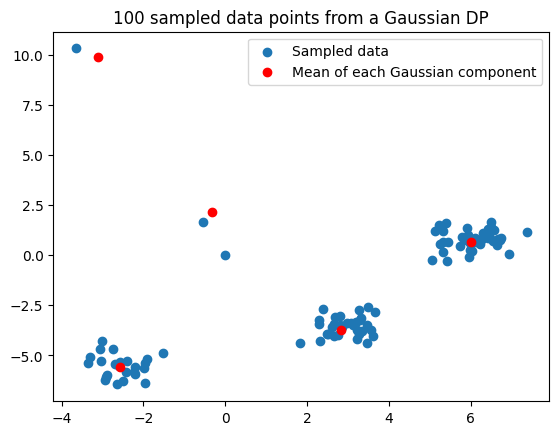
\includegraphics[scale=0.5]{images/sampled_dataset.png}
    \caption{Dataset sampled}
    \label{fig:data_sampl}
\end{figure}

\subsection{Implementing the VI algorithm}
To implement the variational inference DP mixture algorithm, we had to make some additional assumptions :

First, we needed to choose a distribution among the one of the exponential family to get closed formulas for
$$p\left(x_n \mid z_n, \boldsymbol{\eta}^*\right)=\prod_{i=1}^K\left(h\left(x_n\right) \exp \left\{\eta_i^{* T} x_n-a\left(\eta_i^*\right)\right\}\right)^{z_n^i}$$ and $$p\left(\eta^* \mid \lambda\right)=h\left(\eta^*\right) \exp \left\{\lambda_1^T \eta^*+\lambda_2\left(-a\left(\eta^*\right)\right)-a(\lambda)\right\}$$.

As the sampled data is known to be generated according to a Gaussian-Gaussian DP mixture, we decided to set every component of the mixture as Gaussian with fixed variance $\sigma^2$ as well.
\\\\
Identifying the parameters reveals that for all \(i\) in \(\{1, \ldots, K\}\), the \(i\)-th component follows a Gaussian distribution with mean \(\sigma^2\eta^*_i\) and covariance matrix \(\sigma^2\mathbb{I}\). \\
It follows that \(\eta^*\) follows a Gaussian distribution with mean \(\lambda_1 / \lambda_2\) and covariance matrix \((1/\lambda_2)\mathbb{I}\).
It also gives that \(a(\eta^*) = \frac{\eta^{*T}\eta^*}{2}\), which is necessary to update the parameters of the multinomial law of \(Z\).\\

\textbf{Note :} The data points and \(\eta^*\) have the same dimension. \(\lambda_1\) has the dimension of \(\eta^*\), and \(\lambda_2\) is a real number.\\

Regarding variational densities and using same identification as before, we also set \(q(\eta_i^* \mid \tau_i)\) to be Gaussian distributions with mean \(\frac{\tau_{i1}}{\tau_{i2}}\) and covariance matrix \(\left(\frac{1}{\tau_{i2}}\mathbb{I}\right)\), where $\tau_i = (\tau_{i1}, \tau_{i2})$ and $\tau_{i1}$ has the dimension of $\eta_i^*$ and $\tau_{i2}$ is a real number.\\

Those equivalents will be required to estimate the density of the data given the parameters of the variational estimated density and to update the parameters while running the algorithm.

We also made sure that our algorithm was working with 2-dimensional data (the sampled data) and 8-dimensional data (the robot data). Further, we made it work regardless the dimension of the data to have the most general implementation possible.

We also tried our best to have an efficient algorithm, by avoiding loop cascades and using the operations built into the torch and numpy modules.

\subsection{Setting the value of hyper parameters}

The hyper parameters of this algorithm are :

\begin{itemize}
    \item the fixed variance $\sigma^2$ of the data (according to the assumption of the model)
    \item $\lambda = (\lambda_1, \lambda_2)$, the parameters of the distribution of $\eta^*$
    \item $\alpha$, the second parameter of the law of the $V_i$.
\end{itemize}

\subsubsection{For the sampled DP mixture}
The hyper parameters of this dataset are easy to set, as we know the underlying structure of the data.
Hence, we will have :

\begin{itemize}
    \item $\sigma^2 = 0.3$
    \item $\lambda_1 = \mathbb{E}_{G_0}[\eta^*] / \text{Var}_{G_0}[\eta^*] = (0, 0)$
    \item $\lambda_2 = 1 / \text{Var}_{G_0}[\eta^*] = 1/10$
\end{itemize}

For the dataset provided in the report above, we found that $\alpha = 0.5$ gave relevant results, but the choice is arbitrary and could be made using grid search, for instance.

Following indications of the paper, we set $$$$

\subsubsection{For the robot data}
We load the Robot data from an external file. Thus, we don't have as much information as for the sampled data.

According to the paper, the covariance matrix is set to be the sample covariance, and the mean of the hyper parameter $\lambda$ is the
sample mean.

Hence, we have :

\begin{itemize}
    \item $\sigma^2 = $ empirical variance
    \item $\lambda_1 =$ empirical mean / empirical variance
    \item $\lambda_2 =$ 1 / empirical variance
\end{itemize}

The mean and variance parameters are computed using only the training data points of the robot data. \\

After testing with different values, we set $\alpha = 0.1$, which an arbitrary choice giving a good ELBO value.


\subsection{Estimating the density of the data}

Once the algorithm successfully gave us the parameters for the posterior distribution, we needed to approximate the distribution of the dataset to be able to compare our result to the data.

For that, we used the following formula, provided in the paper :

$$p\left(x_{N+1} \mid \mathbf{z}, \alpha, \lambda\right)=\sum_{i=1}^K \mathrm{E}\left[\theta_i \mid \gamma\right] p\left(x_{N+1} \mid \tau_i\right)$$, where $p\left(x_{N+1} \mid \tau_i\right)$ is the $i$-th component of $p\left(x_n \mid z_n, \boldsymbol{\eta}^*\right)$ where $\eta_i^*$ is replaced by its mean, computed using the VI algorithm, which is $$\tau_{i1} / \tau_{i2}$$.

\section{Result}

There are a number of points to note about the obtained results.

\begin{figure}[H]
    \begin{minipage}{0.45\textwidth}
        \centering
        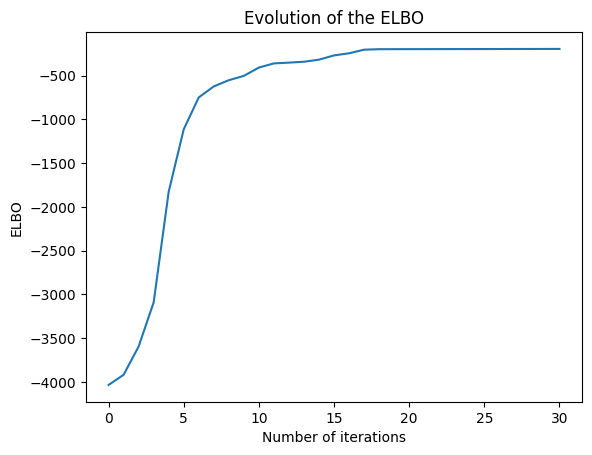
\includegraphics[scale=0.3]{images/elbo_sampled.png}
        \caption{ELBO evolution for the fitting on the simulated data}
        \label{fig:elbo_sim}
    \end{minipage}\hfill
    \begin{minipage}{0.45\textwidth}
        \centering
        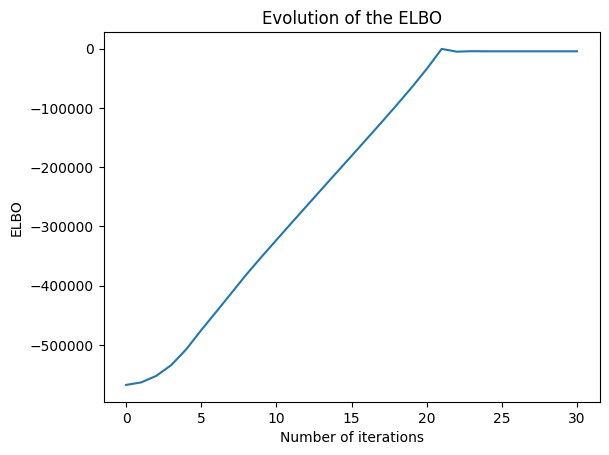
\includegraphics[scale=0.3]{images/Robot_Elbo.png}
        \caption{ELBO evolution for the fitting on the robot data}
        \label{fig:elbo_rob}
    \end{minipage}
\end{figure}

Firstly, we can see that the entropy converges quickly. It takes approximately 17 iterations to converge to the generated synthetic data as we can see in the figure \ref{fig:elbo_sim}, and approximately 22 iterations to converge to the robot data [\ref{fig:elbo_rob}. Running on a personal computer, the model takes about 0.6 seconds to converge to the synthetic data, and 2 minutes 30 seconds for the robot data.

\begin{figure}[H]
    \centering
    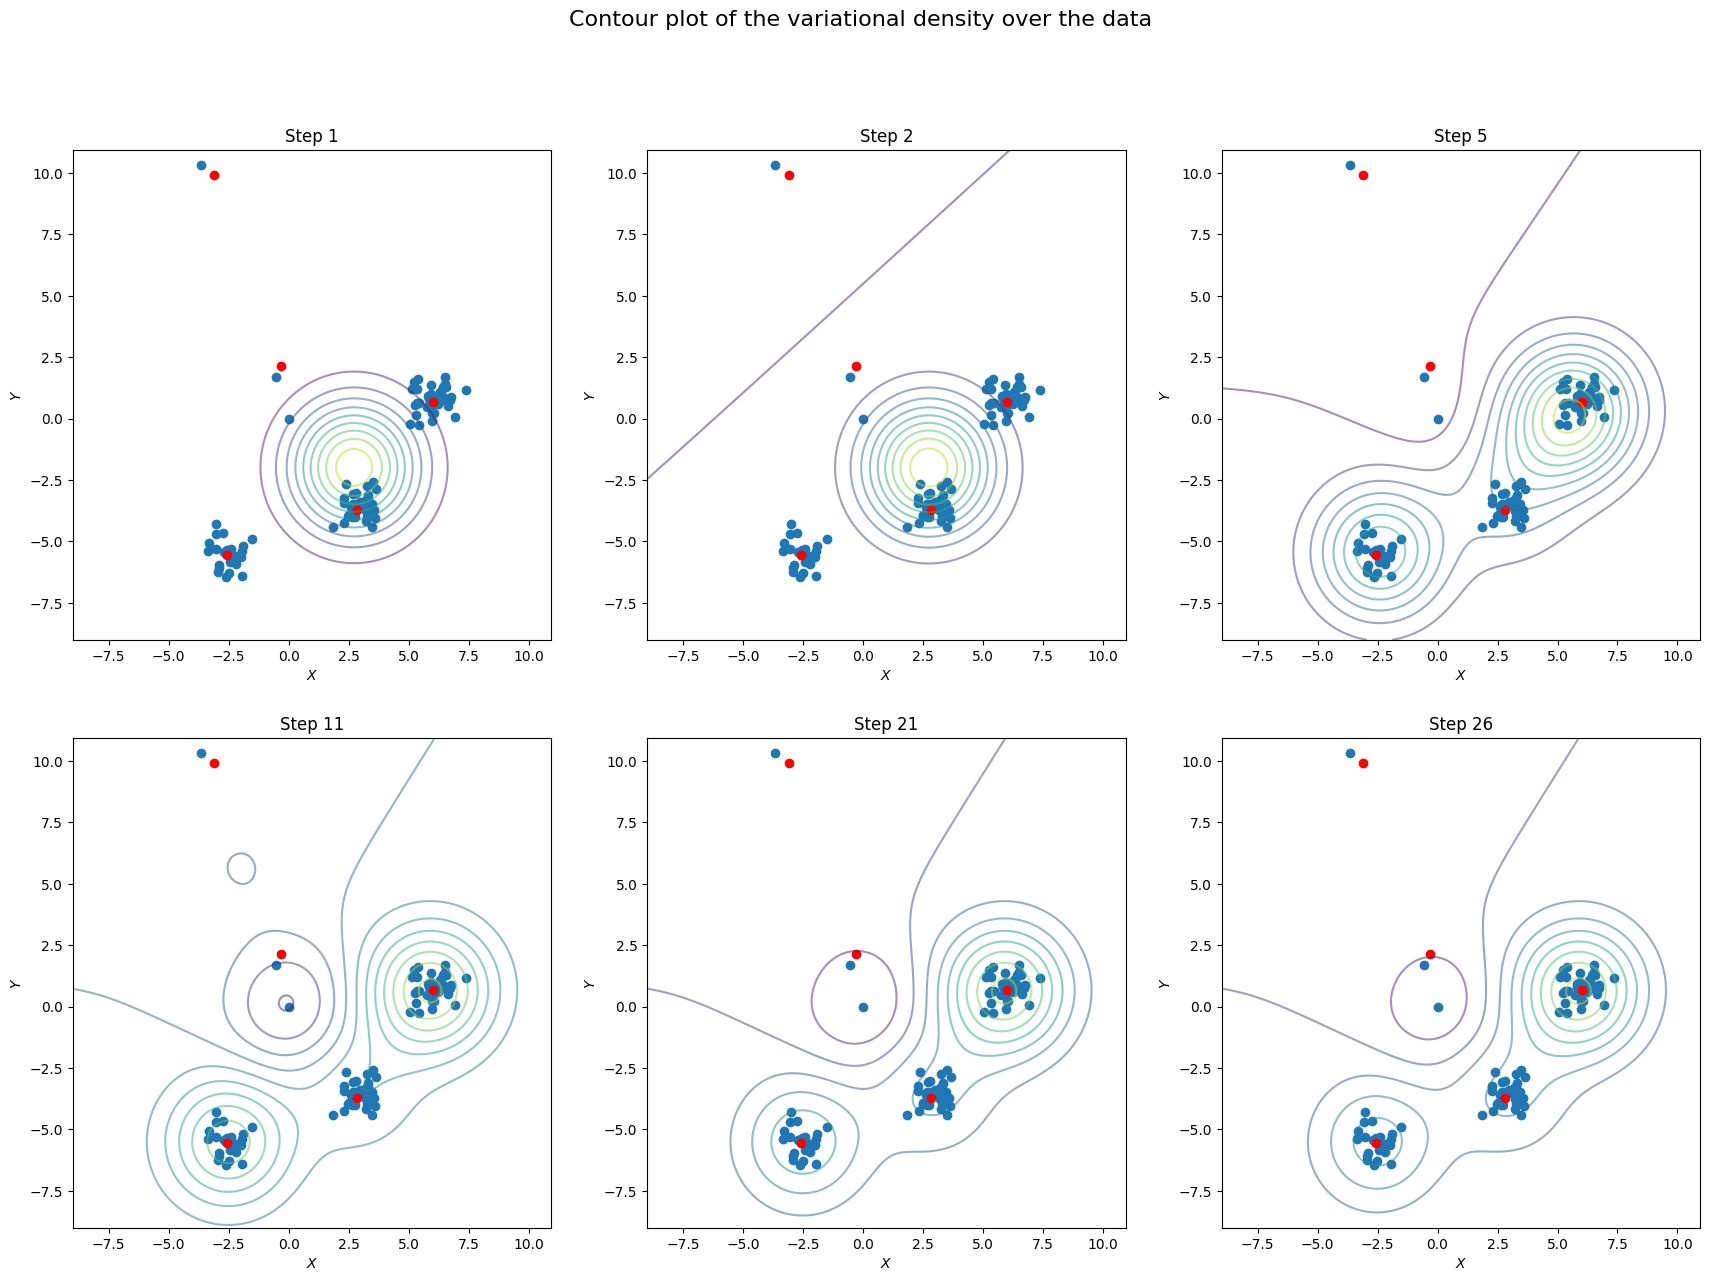
\includegraphics[scale=0.4]{images/sampled_evolution.png}
    \caption{Evolution of the parameters' update for the simulated data}
    \label{fig:alg_evol}
\end{figure}

\begin{figure}[H]
    \centering
    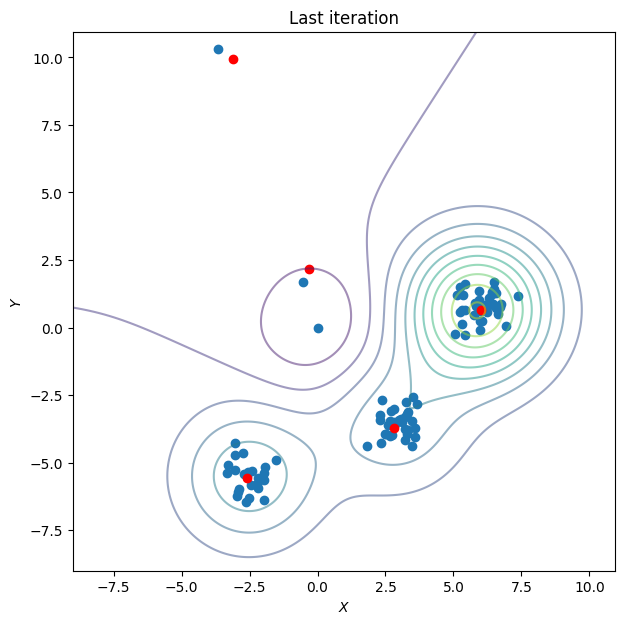
\includegraphics[scale=0.4]{images/sampled_last_iteration.png}
    \caption{Last iteration result for the simulated data}
    \label{fig:alg_last}
\end{figure}
\begin{figure}[H]
    \centering
    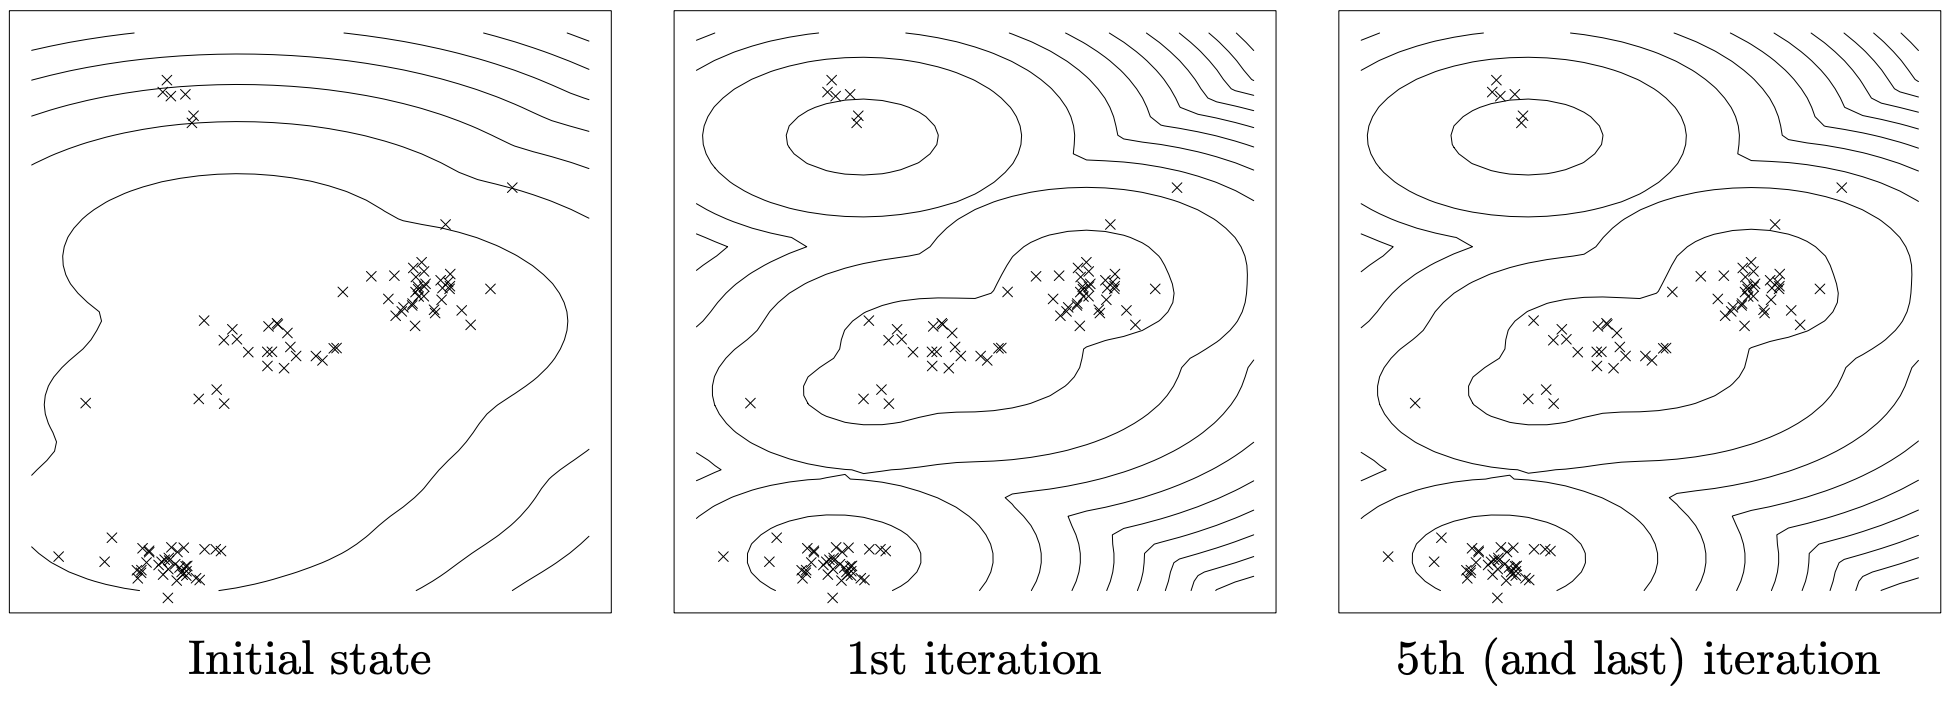
\includegraphics[scale=0.4]{images/paper_result.png}
    \caption{Result obtained in the original paper}
    \label{fig:alg_paper}
\end{figure}

Secondly, now on the simulated data, we can see that the algorithm gives good results on the figure \ref{fig:alg_last}, similarly to that of the paper (figure \ref{fig:alg_paper}) but it seems to converge a little bit slower. Indeed, in the paper, they stopped the algorithm to 5 iterations and even if we had great result at 5 iterations we did 30 iterations to get better results.
The approximated density fits the data closely. Indeed, we can see that the algorithm well identifies 3/4 clusters. We can see that in areas where the points are less agglomerated, the more the contours turn to violet, indicating a lower density of expected values, and vice versa. Like in the paper, for the cluster of points that is between two well separated clusters, we can see that the density is combining like it is expected. Moreover, the algorithm predicts two well defined clusters easily identified when we see the dataset. Overall the algorithm works well and was used to create an accurate reproduction of the results obtained in the paper.

\subsection{Held-out log-likelihood}
One last step to evaluate the performances of the model is to compute its held-out log-likelihood and its training time.

As done in the paper, we did it for data whose the dimension goes from 5 to 50. Thus, we needed to generate data points with higher dimension than 2. For that, we used the function \textbf{multivariate\_normal} from \textbf{numpy.random}, and we adjusted the dimension of the mean and the covariance matrix. We also made sure that our CAVI algorithm could be used for higher dimension than 2.

To build the held-out sets, we used the train set to which we added a Gaussian noise, with two times the variance of the training set.

An example of held out set is shown below, in two dimensions :

\begin{figure}[H]
    \centering
    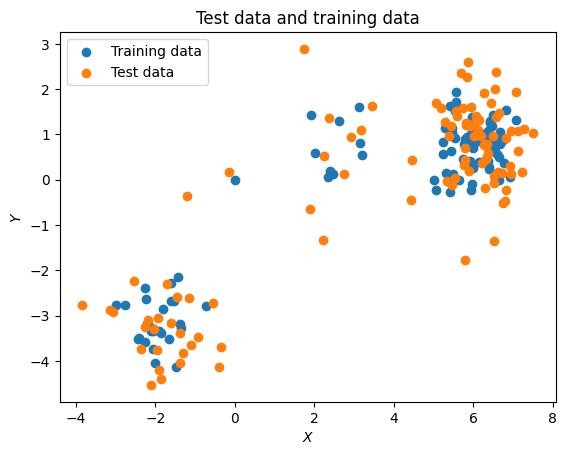
\includegraphics[scale=0.4]{images/held-out_set.png}
    \caption{Example of training and testing sets.}
\end{figure}


The steps done to compute the held-out likelihood and the training time of the model (given the dimension of the input data) are summed up below :

\begin{itemize}
    \item Generate 100 samples of a multivariate Gaussian with the same parameters as above (zero mean and fixed variance of 0.3) for the dimensions 5, 10, 20, 30, 40 and 50,
    \item Perform the CAVI algorithm and compute the estimated density of the data for each dimension, storing the running time,
    \item Generate a held-out set by adding a Gaussian noise to the training set,
    \item Compute the log-density for each point of the test set using the estimated density,
    \item Get the mean of all the computed log-density to get the log-likelihood of the test set.
\end{itemize}

We get the following results concerning the running time and the held-out likelihood :

\begin{figure}[H]
    \centering
    \begin{minipage}{0.5\textwidth}
        \centering
        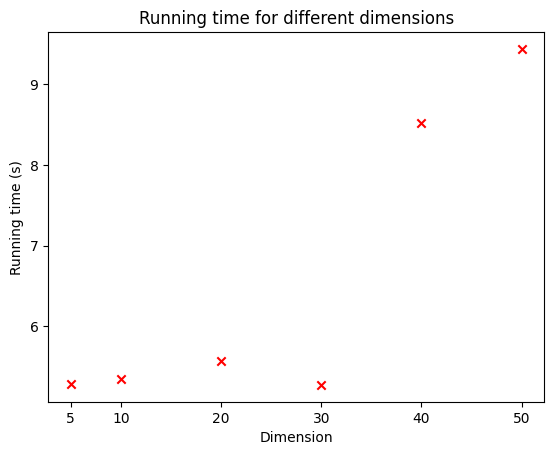
\includegraphics[scale=0.4]{images/running time.png}
        \caption{Running time}
    \end{minipage}%
    \begin{minipage}{0.5\textwidth}
        \centering
        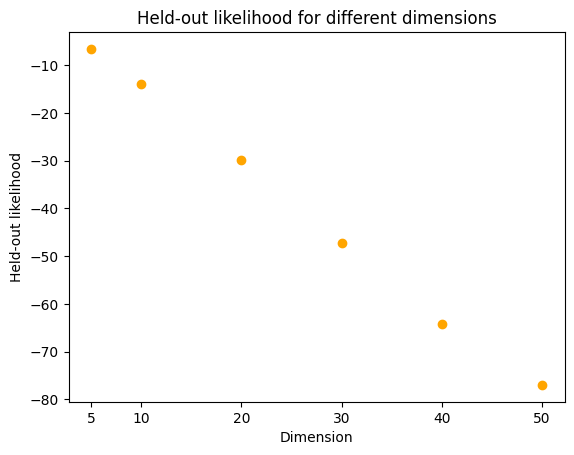
\includegraphics[scale=0.4]{images/held-out likelihood.png}
        \caption{Held-out likelihood}
    \end{minipage}
\end{figure}

We can observe that the running time tends to increase with the dimension of the input data. However, it barely reaches 10 seconds, even for an input data with 50 dimensions. It confirms the results of the paper, which was showing that the variational method was a lot faster to train than the two other tested methods. \\
Concerning the held-out likelihood, we observe the same decreasing trend as in the paper with respect to the dimension. The values of the held-out log-likelihood are different though. It seems normal as the computations details of the held-out likelihood are not precised in the paper. It might take into account constants that we don't compute, for example.


\section{Discussion}

Blei \& Jordan's paper introduces variational inference as an effective strategy to overcome the computational complexities in performing exact Bayesian inference within DP models. The approach used in this paper relies on addressing the challenges posed by the infinite-dimensional nature of the DP and the computational demands of complex Bayesian non-parametric models. Therefore in their approach, the authors deal with the problem of exact inference by using variational inference, which approximates the posterior distribution with a more convenient variational distribution. They work on making this simpler distribution as close as possible to the real one by minimizing the Kullback-Leibler divergence from the true posterior. By doing so, they introduce a computationally feasible method to approximate the posterior distribution over latent variables, such as cluster assignments or mixture parameters, in DP-based models. From the results, we can see that this method provides an excellent trade-off between computational efficiency and accuracy. It allows a model to flexibly choose the form of the approximating variational distribution, thus balancing computational tractability with the closeness of the approximation to the true posterior. This way of working makes it possible to use these models on large sets of information or in complicated situations where it's too complex to model precisely, specifically in situations where exact inference methods might be impractical or infeasible.

To conclude with the approach we can say that by introducing variational inference techniques to approximate the a posteriori distribution in DP-based models, the authors show the possibility of using non-parametric Bayesian statistics It offers a practical way to manage the complexities of these models, making them easier to use in different areas like grouping data, creating mixtures, and estimating densities. This happens by lessening the computer work needed to figure things out exactly in cases where there are endless possibilities, making these models more useful and relevant across various fields.

While the advances made possible by this method cannot be overstated, the paper has a number of flaws that make it difficult to understand and reproduce the results found by the authors; in particular the lack of directly applicable formulas and the abundance of non-explicit parameters and densities. Indeed, throughout the paper, the authors give us many different mathematical formulas, but few of these formulas are directly usable as is, so further research is needed to apply the method computationally. Additionally, the fact that the authors juggle with formulas throughout the article, relying on formulas and explanations stated well in advance of their usefulness, makes it all the more difficult to fully understand the outlined method. The gaps in the specification of experimental parameters make replication of experiments difficult. This imprecision can hamper the validation of results, and give rise to uncertainty as to the robustness of the conclusions drawn from these experiments.

Another problematic aspect is the lack of clarity in the choice of exponential families used. These choices, crucial in probabilistic analysis, lack clear specifications, which can lead to variable interpretations and divergent results. Thus to maximize the practical impact of this document, it could be a good idea to further develop the theoretical explanations with concrete examples, to clarify the choices of exponential families and to specify the experimental parameters exhaustively. This improvement in clarity and specificity would enable a better understanding and more effective use of these methods in real-life applications.

Perhaps further criticism can be made regarding the data used to experiment with the models in the paper. Firstly, when testing with synthetic data, the authors  only use 100 data-points which isn't necessarily enough to get a truly representative sample. Perhaps it would be good to increase the number of synthetic data points generated to test the algorithm. Secondly, concerning the robot data, we have a running time comparison and the likelihood value comparison between using the variational inference method and the Gibbs sampling method. However, the authors provide no visualization of the results compared to the actual robot data. The models are compared to each other, but not with the true distribution.

In sum, "Variational Methods for the Dirichlet Process" represents an important milestone in this area of scientific literature, but validation and experimentation with practical value of the paper remains hampered by the lack of specific details and clearly defined parameters, necessitating further efforts to make its methods more accessible and applicable in real-life contexts.

\end{document}